\section{Performance Evaluation}
\label{sec:ch3_eval}
\subsection{Setup}
Agentless + RepoGraph + CacheBlend
\subsubsection{Metric}
% resolve rate as in RepoGraph original paper, patch application rate optional. 
continue to use resolve rate 

Explanation same as in \ref{sec:ch1_eval}: This metric provides a direct measure of end-to-end task success, capturing not only whether a patch is syntactically correct but also whether it integrates cleanly into the repository and satisfies the intended functionality. Compared to intermediate measures such as code similarity or partial compilation success, the resolve rate reflects the practical utility of the generated patches and therefore serves as a good indicator of real-world performance.

\subsubsection{Datasets}

SWE-bench Verified-mini \cite{MariusHobbhahn2025swe-bench-verified-mini}
%, which is a subset of SWE-bench Verified\cite{chowdhury2024swebenchverified} that is selected via k-means clustering and linear programming, such that the marginal distributions of important scores are preserved. This is a smaller dataset than SWE-bench Lite\cite{yang2024sweagent}, yet high-quality and well-specified, and is capable of reflecting an agent's performance across a spectrum of task difficulties.
\subsubsection{Model}
\label{sec:ch3_eval_model}
Devstral Small hosted on vLLM + LMCache with CacheBlend enabled

\subsection{Results}

\begin{figure}[ht]
\centering
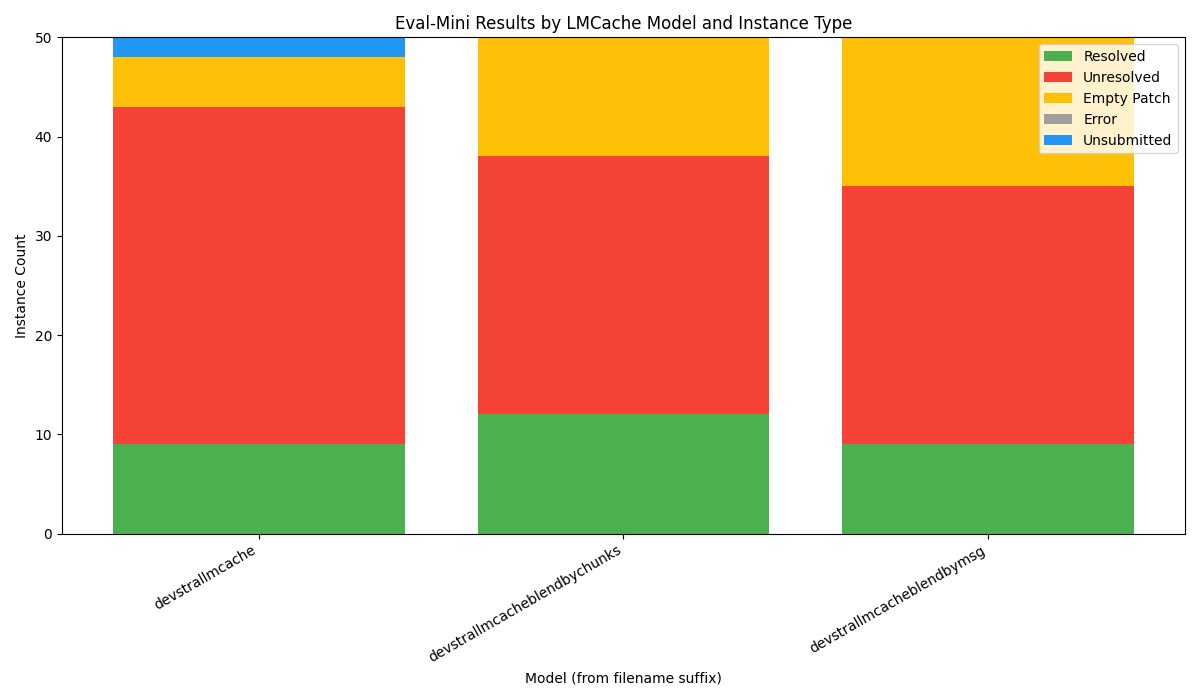
\includegraphics[width=\linewidth]{graphs/visualized_eval_mini_results_lmcache.png}
\vspace{-0.2in}
  \caption{\small Results distributions for SWE-bench Verified-mini evaluation runs across different blending methods, served model is Devstral Small.}
 \label{fig:e2e_blended_perf}
 \vspace{-0.15in}
\end{figure}


% TODO: uncomment when images are available
% \begin{figure}[ht]
% \centering
% 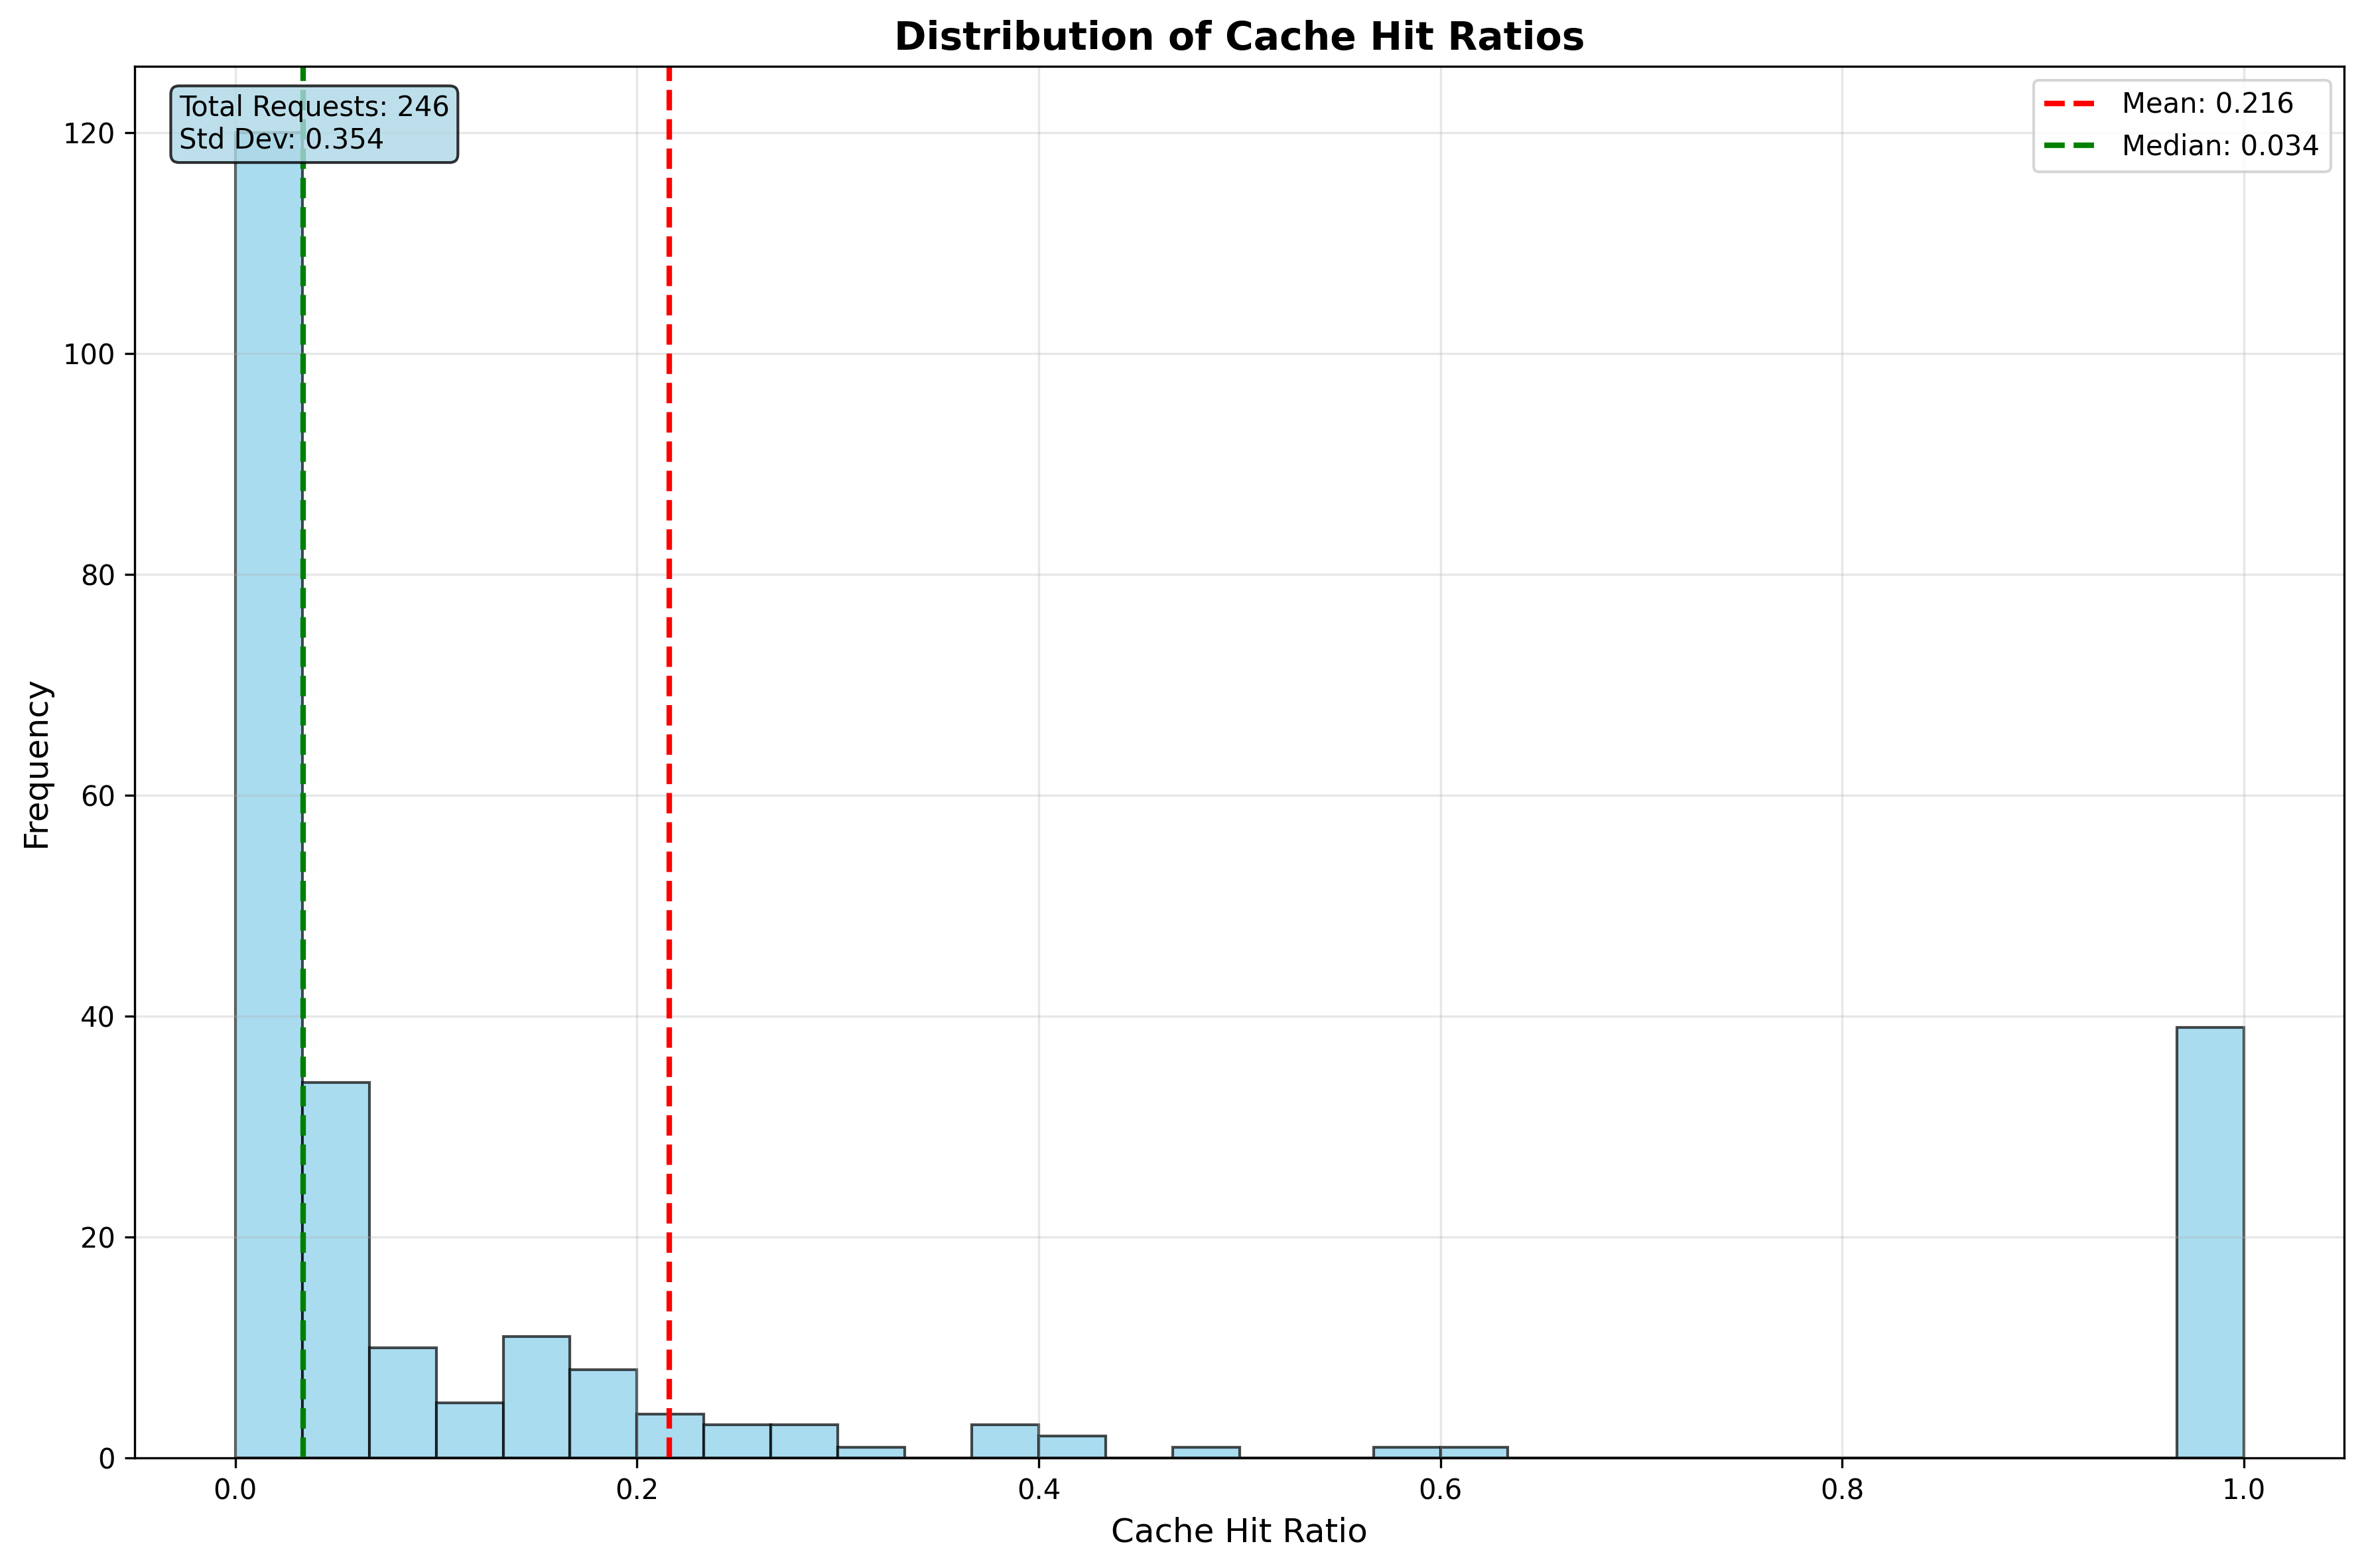
\includegraphics[width=\linewidth]{graphs/hit_ratio_histogram.png}
% \vspace{-0.2in}
%   \caption{\small Hit ratio distribution from running RepoGraph as frontend w/ SWE-bench Verified-mini.}
%  \label{fig:hit_ratio_histogram}
%  \vspace{-0.15in}
% \end{figure}
%
% \begin{figure}[ht]
% \centering
% 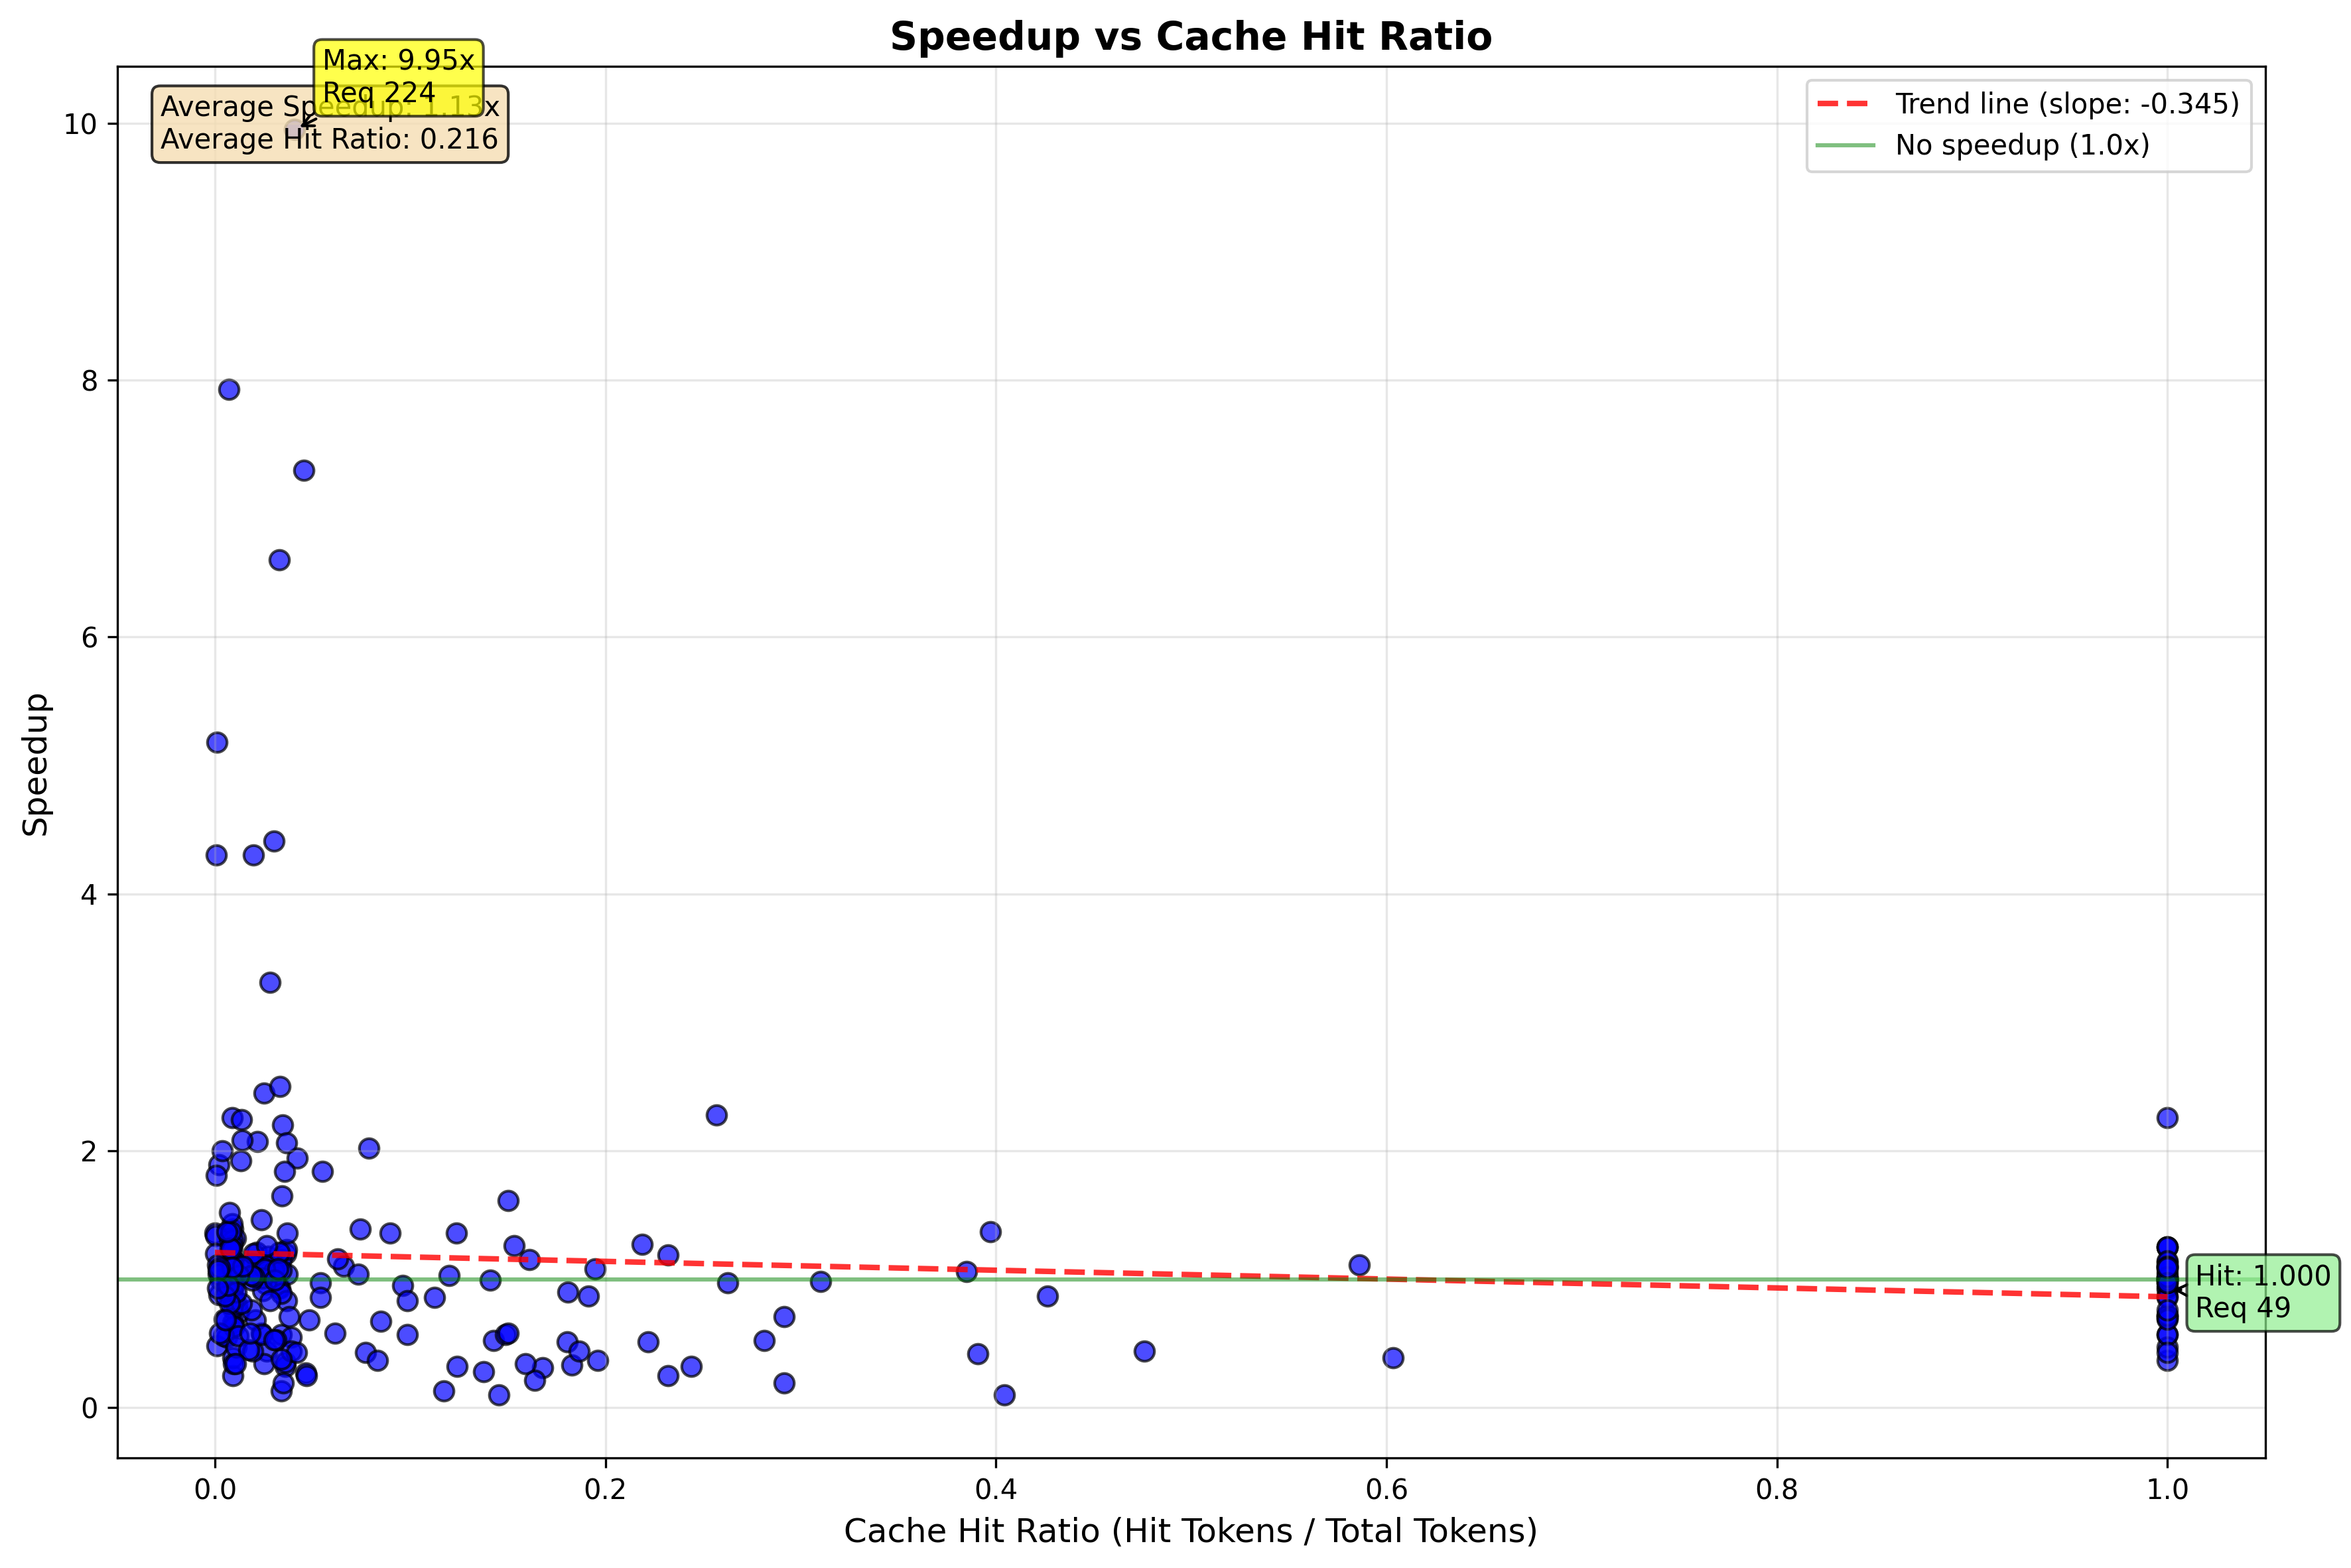
\includegraphics[width=\linewidth]{graphs/hit_ratio_vs_speedup.png}
% \vspace{-0.2in}
%   \caption{\small Hit ratio against overall latency speedup from running RepoGraph as frontend w/ SWE-bench Verified-mini.}
%  \label{fig:hit_ratio_vs_speedup}
%  \vspace{-0.15in}
% \end{figure}